% This is the Reed College LaTeX thesis template. Most of the work
% for the document class was done by Sam Noble (SN), as well as this
% template. Later comments etc. by Ben Salzberg (BTS). Additional
% restructuring and APA support by Jess Youngberg (JY).
% Your comments and suggestions are more than welcome; please email
% them to cus@reed.edu
%
% See http://web.reed.edu/cis/help/latex.html for help. There are a
% great bunch of help pages there, with notes on
% getting started, bibtex, etc. Go there and read it if you're not
% already familiar with LaTeX.
%
% Any line that starts with a percent symbol is a comment.
% They won't show up in the document, and are useful for notes
% to yourself and explaining commands.
% Commenting also removes a line from the document;
% very handy for troubleshooting problems. -BTS

% As far as I know, this follows the requirements laid out in
% the 2002-2003 Senior Handbook. Ask a librarian to check the
% document before binding. -SN

%%
%% Preamble
%%
% \documentclass{<something>} must begin each LaTeX document
\documentclass[12pt,twoside]{reedthesis}
% Packages are extensions to the basic LaTeX functions. Whatever you
% want to typeset, there is probably a package out there for it.
% Chemistry (chemtex), screenplays, you name it.
% Check out CTAN to see: http://www.ctan.org/
%%
\usepackage{graphicx,latexsym}
\usepackage[french]{babel} 
\usepackage{amsmath}
\usepackage{amssymb,amsthm}
\usepackage{xcolor}
\usepackage{eso-pic}
\usepackage{longtable,booktabs,setspace}
\usepackage{chemarr} %% Useful for one reaction arrow, useless if you're not a chem major
\usepackage[hyphens]{url}
\usepackage{tikz}
\usetikzlibrary{calc}
\newcommand\HRule{\rule{\textwidth}{1pt}}
% Added by CII
\usepackage{hyperref}
\usepackage{lmodern}
\usepackage{float}
\floatplacement{figure}{H}
% End of CII addition
\usepackage{rotating}

% Next line commented out by CII
%%% \usepackage{natbib}
% Comment out the natbib line above and uncomment the following two lines to use the new
% biblatex-chicago style, for Chicago A. Also make some changes at the end where the
% bibliography is included.
%\usepackage{biblatex-chicago}
%\bibliography{thesis}


% Added by CII (Thanks, Hadley!)
% Use ref for internal links
\renewcommand{\hyperref}[2][???]{\autoref{#1}}
\def\chapterautorefname{Chapter}
\def\sectionautorefname{Section}
\def\subsectionautorefname{Subsection}
% End of CII addition

% Added by CII
\usepackage{caption}
\captionsetup{width=5in}
% End of CII addition

% \usepackage{times} % other fonts are available like times, bookman, charter, palatino


% To pass between YAML and LaTeX the dollar signs are added by CII
\title{THÈSE}
\author{Thomas Karaouzene}
\labo{}
% The month and year that you submit your FINAL draft TO THE LIBRARY (May or December)
\date{31 octobre 2017}
\division{}
\advisor{Pierre Ray}
%If you have two advisors for some reason, you can use the following
% Uncommented out by CII
\altadvisor{Nicolas Thierry-Mieg}
% End of CII addition

%%% Remember to use the correct department!
\department{Ingénierie de la Santé, de la Cognition et Environnement (EDISCE)}
% if you're writing a thesis in an interdisciplinary major,
% uncomment the line below and change the text as appropriate.
% check the Senior Handbook if unsure.
%\thedivisionof{The Established Interdisciplinary Committee for}
% if you want the approval page to say "Approved for the Committee",
% uncomment the next line
%\approvedforthe{Committee}

% Added by CII
%%% Copied from knitr
%% maxwidth is the original width if it's less than linewidth
%% otherwise use linewidth (to make sure the graphics do not exceed the margin)
\makeatletter
\def\maxwidth{ %
  \ifdim\Gin@nat@width>\linewidth
    \linewidth
  \else
    \Gin@nat@width
  \fi
}
\makeatother

\renewcommand{\contentsname}{Table of Contents}
% End of CII addition

\setlength{\parskip}{0pt}

% Added by CII

\providecommand{\tightlist}{%
  \setlength{\itemsep}{0pt}\setlength{\parskip}{0pt}}

\Acknowledgements{

}

\Dedication{

}

\Preface{
This is an example of a thesis setup to use the reed thesis document
class (for LaTeX) and the R bookdown package, in general.
}

\Abstract{

}

% End of CII addition
%%
%% End Preamble
%%
%

\usepackage{amsthm}
\newtheorem{theorem}{Theorem}[section]
\newtheorem{lemma}{Lemma}[section]
\theoremstyle{definition}
\newtheorem{definition}{Definition}[section]
\newtheorem{corollary}{Corollary}[section]
\newtheorem{proposition}{Proposition}[section]
\theoremstyle{definition}
\newtheorem{example}{Example}[section]
\theoremstyle{remark}
\newtheorem*{remark}{Remark}
\begin{document}

% Everything below added by CII
      \maketitle
  
  \frontmatter % this stuff will be roman-numbered
  \pagestyle{empty} % this removes page numbers from the frontmatter

  
      \begin{preface}
      This is an example of a thesis setup to use the reed thesis document
      class (for LaTeX) and the R bookdown package, in general.
    \end{preface}
  
      \hypersetup{linkcolor=black}
    \setcounter{tocdepth}{2}
    \tableofcontents
  
      \listoftables
  
      \listoffigures
  
  
  
  \mainmatter % here the regular arabic numbering starts
  \pagestyle{fancyplain} % turns page numbering back on

  \chapter*{Remerciements}\label{remerciements}
  \addcontentsline{toc}{chapter}{Remerciements}
  
  Je remercie \ldots{}
  
  \newpage  
  
  ~
  
  ~
  
  ~
  
  ~
  
  ~
  
  ~
  
  ~
  
  ~
  
  ~
  
  ~
  
  ~
  
  ~
  
  ~
  
  ~
  
  ~
  
  ~
  
  ~
  
  ~
  
  ~
  
  ~
  
  ~
  
  ~
  
  ~
  
  ~
  
  ~
  
  ~
  
  ~
  
  ~
  
  ~
  
  ~
  
  ~
  
  ~
  
  ~
  
  ~
  
  ~
  
  ~
  
  ~
  
  ~
  
  ~
  
  ~
  
  ~
  
  ~
  
  ~
  
  \begin{verbatim}
                        Cette thèse est dédiée à ...
  \end{verbatim}
  
  \chapter*{Résumé}\label{resume}
  \addcontentsline{toc}{chapter}{Résumé}
  
  The preface pretty much says it all. \par
  
  Second paragraph of abstract starts here.
  
  \chapter*{Abstract}\label{abstract}
  \addcontentsline{toc}{chapter}{Abstract}
  
  The preface pretty much says it all. \par
  
  Second paragraph of abstract starts here.
  
  \chapter{Introduction}\label{introInf}
  
  \section{La spermatogénèse}\label{la-spermatogenese}
  
  La spermatogenèse des mamifères est un processus long et complexe
  controllé par plusieurs mécanismes étroitement liés ((Gnessi, Fabbri, \&
  Spera, 1997, Kierszenbaum (1994)),\textbf{Sharpe1994 à trouver!!!}).
  C'est au cours de celle-ci que, à partir de cellules germinales, seront
  produits les spermatozoïdes matures. Ce processus est divisé en trois
  phases principales : La phase de multiplication, la phase de division
  (appelée la méiose) et la phase de maturation. Chez les hommes, ces
  tapes se déroulent en continue dans la paroi des tubes séminifères du
  testicules depuis la pubertés jusqu'à la mort et implique trois types de
  cellules germinales : les spermatogonies, les spermatocytes et les
  spermatides. Le temps nécessaire pour obtenir un spermatozoïde mature à
  partir de cellules germinales est de 74 jours et la production
  quotidienne de spermatozoïde est d'environ 45 million par testicules
  (Johnson, Petty, \& Neaves, 1980).
  
  \subsection{Rappels sur le testicule}\label{rappels-sur-le-testicule}
  
  Les testicules sont les organes sexuels masculins. Ils possèdes deux
  fonctions principales plus ou moins exprimés selon les période de la vie
  de l'individu : une fonction endocrine caractérisé par la synthèse des
  hormones stéroïdes sexuelles masculines (la stéroïdogenèse) et une
  fonction exocrine au cours de laquelle seront produits les gamètes
  masculins. Chez un individu adulte en bonne santé, celui-ci présente une
  forme ovoïde ayant un volume moyen de 18
  cm\textsuperscript{\textsuperscript{3}} par testicule. Comme chez la
  plupart des mammifères terrestres, ils sont sous le pénis dans dans une
  poche de peau appelée scrotum et reliés à l'abdomen par le cordon
  spermatique (\textbf{Figure :} \ref{fig:testicule}). Cette
  externalisation des testicules permet leur maintien à une température
  plus basse que celle du reste du corps nécessaire à la spermatogenèse.\\
  L'intérieur du testicule contient des tubes séminifères enroulés ainsi
  que du tissu entre les tubules appelé espace interstitiel. Les tubes
  séminifères sont de longs tubes compactés sous forme de boucles et dont
  les deux extrémités débouchent sur le \emph{rete testis} (\textbf{Figure
  :} \ref{fig:testicule}). C'est le long des parois du tube séminifère que
  se dérouleront l'ensemble des étapes de la spermatogenèse.
  
  \begin{figure}
  
  {\centering 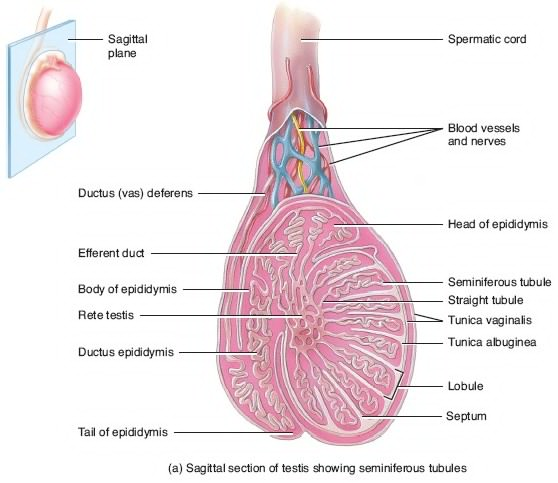
\includegraphics[scale=0.65]{figure/coupe_testicule2} 
  
  }
  
  \caption{Schéma anatomique du testicule humain : }\label{fig:testicule}
  \end{figure}
  
  \subsection{La phase de
  multiplication}\label{la-phase-de-multiplication}
  
  La phase de multiplication est la phase au cours de laquelle les
  spermatogonies se divisent par mitoses pour aboutir au stade de
  spermatocytes primaires. Les spermatogonies sont des cellules dploïdes à
  l'origine de k'ensemble des autres cellules germinales humaines. Pour
  cela, elle vont s'auto-renouveller par mitose successive afin de
  maintenir une production continue de spermatozoïdes tout au long de la
  vie de l'individu. Ces cellules sont localisées dans le compartiment
  basal des tubes séminifères. Elles présentent un noyau ovoïde ainsi
  qu'un cytoplasme dense contenant un petit appareil de Golgi, quelques
  mitochondrie ainsqi que plusieurs ribosomes libres. Les analyses
  histologiques ont permis de distinguer trois types de spermatogonies en
  fonction de leur contenu en heterochromatine ((Clermont, 1963, Clermont
  (1966), Goossens \& Tournaye (2013))) :
  
  \begin{enumerate}
  \def\labelenumi{\arabic{enumi}.}
  \tightlist
  \item
    Les spermatogonies de type A dark (ou Ad)\\
  \item
    Les spermatogonies de type A pale (ou Ap)\\
  \item
    Les spermatogonies de type B
  \end{enumerate}
  
  Chez l'Homme, les spermatogonies Ad ont une activité mitotique au cours
  de la spermatogénès et servent de résèrve. Elles vont au cours d'une
  première mitose former un spermatogonie Ad et un spermatogonie Ap
  (\textbf{Figure :} \ref{fig:spermatogenese}). Cette propriété permet à
  la fois de se différencier en spermatocytes tout en constituant un
  compartiment de réserve de spermatogonies Ad pour la regénération de la
  population de cellules germinales au sein de l'épithelium séminifère.
  L'entrée en division des spermatogonies Ap se fait par groupes
  cellulaire tout les 16 jours. Les Cellules d'une même génération
  maintiennent entre elles des ponts cytoplasmiques jusqu'à la
  spermiogénèse ce qui permet la synchronisation parfaite du développement
  gamétique de toutes les cellules filles issues d'un groupe de
  spermatogonies Ap. Ce phénomène est appelé onde spermatogénétique.
  Chaque spermatogonies Ap va, lorsqu'ils se divise par mitose, former
  deux spermatogonies B qui eux-mêmes se diviseront en deux spermatocytes
  primaires diploïdes (\textbf{Figure :} \ref{fig:spermatogenese}).
  
  \begin{figure}
  
  {\centering 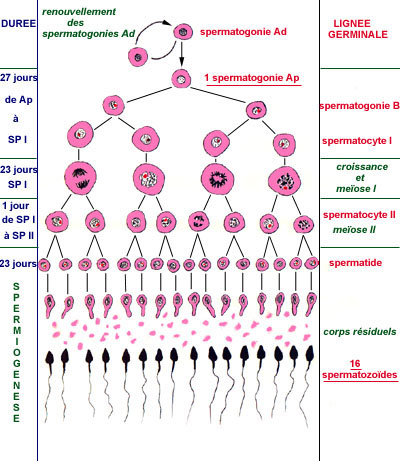
\includegraphics[scale=0.75]{figure/spermatogenese} 
  
  }
  
  \caption{Les différentes phases de la spermatogénèse}\label{fig:spermatogenese}
  \end{figure}
  
  \subsection{La méïose}\label{la-meiose}
  
  La méiose, ou phase de maturation, est l'étape au cours de laquelle, à
  partir de cellules diploïdes (les spermatogonies B) vont se former des
  cellules haploïdes, les spermatocytes secondaire (spermatocytes II). Ce
  résultat est le fruit de deux divisions succesives (\textbf{Figure :
  }\ref{fig:meiose}) appellée respectivement méïose réductionnelle ou
  méiose I (MI) et méiose équationnelle ou méiose II (MII). La MI va
  séparer les chromosomes homologues, produisant deux cellules et
  résuisant la ploïdie de diploïde à haploïde (d'où son non
  \emph{réductionelle}). En plus de son rôle de division vu précédement,
  la méiose joue un rôle clef dans le brassage génétique (mélange des
  gènes) et ce, grâce à deux mécanismes de brassage : le brassage
  interchromosomique, lorsque les chromosomes sont séparés et le brassage
  intrachromosomique inpliquant nottament des enjambements chromosomiques
  (crossing-over) (\textbf{Figure : }\ref{fig:crossingover}).
  
  \begin{figure}
  
  {\centering 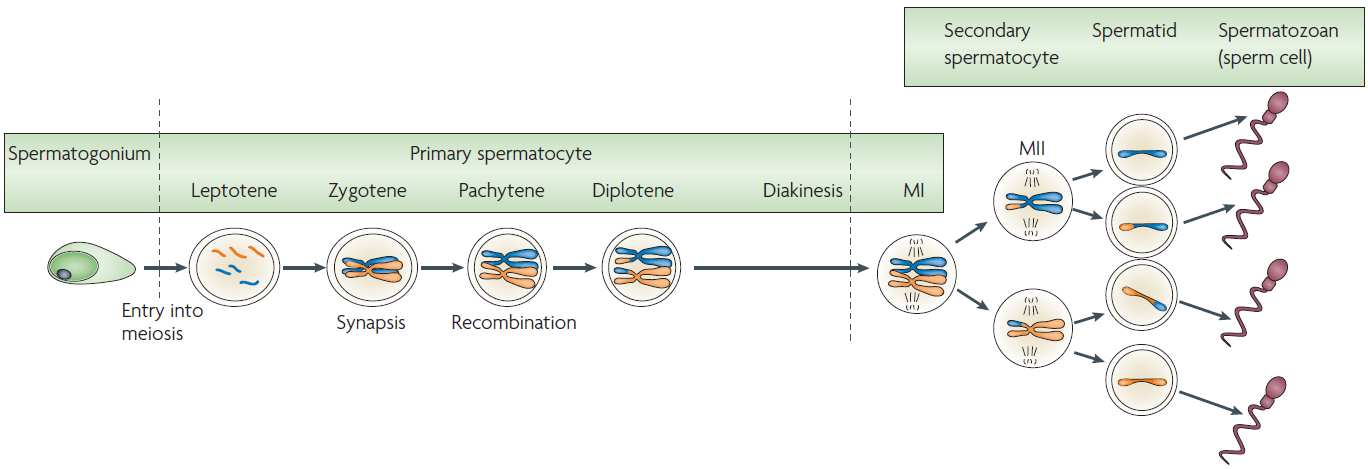
\includegraphics[scale=0.35]{figure/Meiosis_Stages} 
  
  }
  
  \caption{Les différentes étapes de la méiose gamétique masculine. D’après Sasaki et Matsui,
  2008}\label{fig:meiose}
  \end{figure}
  
  La méiose est initié dès la fin de la phase de multiplication à partir
  des spermatocytes primaires issus de la division des spermatogonies de
  type B. Ces cellules nouvellement formées se situent dans le
  compartiment basal du tube séminifère. C'est là qu'ils vont tout d'abord
  subir une interphase (stade préleptotène) durant entre 2 à 4 jours. Au
  cours de cette phase a lieu la réplication de l'ADN. Cette réplication
  se fait lorsque l'ADN est à l'état de chromatine, pendant la phase S
  (pour syntèse) de l'interphase. À l'issus de cette phase, chaque
  chromosome sera composé de deux chromatides reliées entres elles par le
  centomère, le materiel génétique de chaque cellules ayant donc été
  multiplié par 2. Par la suite, ces cellules vont subir deux divisions
  méiotiques, chacune composées de 4 étapes distincte (\textbf{Figure :
  }(\ref{fig:mitose})) :
  
  \begin{enumerate}
  \def\labelenumi{\arabic{enumi}.}
  \tightlist
  \item
    La prophase, caractérisée par la condentation de la chromatine formant
    ainsi les chromosome\\
  \item
    La métaphase, phase au cours de laquelle les chromosomes vont
    s'aligner à l'equateur de la cellule pour former la plaque
    équatoriale\\
  \item
    L'anaphase, les chromatides soeurs (ou les chromosomes homologues en
    fonction de la phase méiotique) vont se séparer et migrer aux pôles
    opposés de la cellule\\
  \item
    La télophase, qui est l'étape finale, les chromosomes se décondensent
    et l'enveloppe nucléaire se reforme autours des chromosomes. La
    cellule mère se sépare alors en deux cellules filles
  \end{enumerate}
  
  \begin{figure}
  
  {\centering 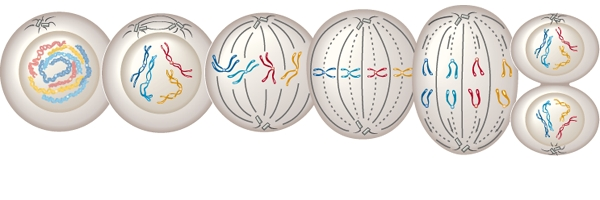
\includegraphics[scale=.5]{figure/phases_mitose} 
  
  }
  
  \caption{Les différentes phases de la division cellulaire : De la prophase (à gauche) à la télophase (à droite) }\label{fig:mitose}
  \end{figure}
  
  La première division méiotique abouti à la formation des spermatocytes
  secondaires (spermatocytes II). À ce states, les cellules sont haploïdes
  et chaque chromosome est composé de deux chromatides soeurs. Après,
  cette brèves étape (environ 1 jour) ainsi qu'une très courte interphase
  sans réplication de l'ADN, les spermatocytes II vont entrer en deuxième
  division méiotique. Cette deuxième division est très semblable à une
  division mitotique. La prophaseII, à la différence de la prophase I, est
  très courte. Lors de cette étape, les chromosomes constitués de
  chromatides sœurs se dirigent vers la plaque équatoriale. En métaphase
  II, les chromosomes s'alignent au niveau de leurs centromères. En
  anaphase II, le centromère de chaque chromosome se rompt séparant les
  chromatides sœurs l'une de l'autre et permettant leur déplacement vers
  les pôles opposés des spermatocytes II. Lors de la télophase II, on
  observe la formation de cellules filles haploïdes appelées spermatides,
  contenant chacune n chromosomes.
  
  \begin{figure}
  
  {\centering 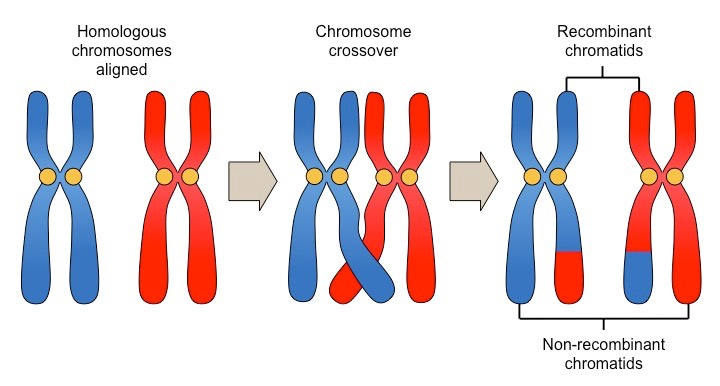
\includegraphics[scale=0.35]{figure/crossingover} 
  
  }
  
  \caption{Schéma simplifé d'un enjambement chromosomique}\label{fig:crossingover}
  \end{figure}
  
  \subsection{La spermiogénèse}\label{la-spermiogenese}
  
  La spermiogénèse est la phase finale de la spermatogénèse. Elle dure
  environs 23 jours chez l'humain et peut être subdivisée en plusieurs
  étapes (\textbf{Figure : }(\^{}ref(fig:spermiogénese))). La
  spermiogénèse définie la cytodiférentiation des spermatides en
  spermatozoïdes. C'est au cours de cette phase que les caractéristiques
  morphologique et fonctionelles du spermatozoïdes seront déterminées
  (Clermont \& Oko 1993 à trouver !!!). Elle est caractérisée par 3
  évènements majeurs : la formation de l'acrosome, la compaction de l'ADN
  nucléaire, la formation de l'acrosome et la formation du flagelle. Le
  développement de l'acrosome et la formation du flagelle commence au
  niveau des spermatides rondes (Escalier et al., 1991) pendant
  l'élongation du spermatide, le noyau se condense et devient hautement
  polarisé (Hamilton, Waites, Special Programme of Research, Family Health
  International (Organization), \& World Health Organization., 1987).\\
  
  \begin{figure}
  
  {\centering 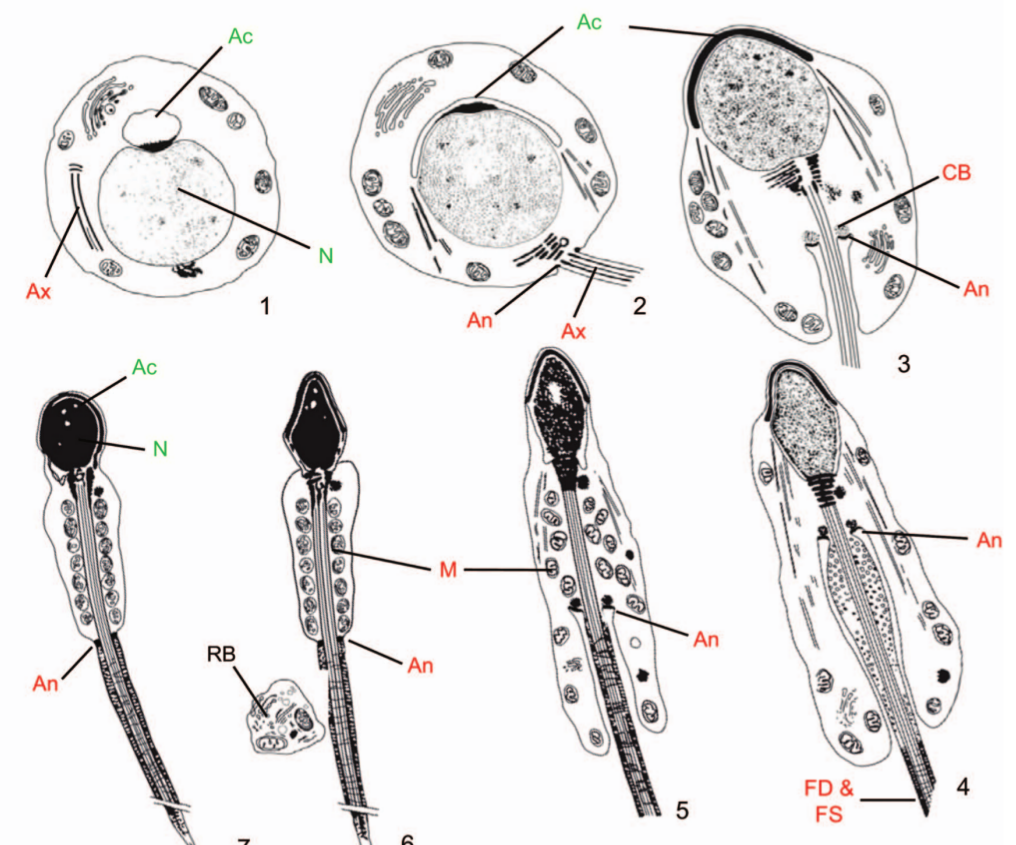
\includegraphics[scale=0.3]{figure/spermiogenese} 
  
  }
  
  \caption{Principales étapes et modifications structurales lors de la spermiogénèse.
  1. La spermatide immature avec un gros noyau arrondi. La vésicule acrosomale est attachée
  au noyau, l’ébauche du flagelle n’atteint pas le noyau. 2. La vésicule acrosomale a augmenté
  de taille et apparaît aplatie au niveau du noyau. Le flagelle entre en contact avec le noyau. 3-
  7. Formation de l’acrosome, condensation du noyau et développement des structures
  flagellaires. Ac, acrosome; Ax, axonème; CC, corps chromatoïdes; CR, corps résiduel; FD,
  fibres denses; GF, gaine fibreuse; M, mitochondrie; Ma, manchette. D’après Touré et al.,
  2011}\label{fig:spermiogénese}
  \end{figure}
  
  \section{Structure et fonction du
  spermatozoïde}\label{structure-et-fonction-du-spermatozoide}
  
  \subsection{Anatomie du spermatozoïde}\label{anatomie-du-spermatozoide}
  
  \begin{figure}
  
  {\centering 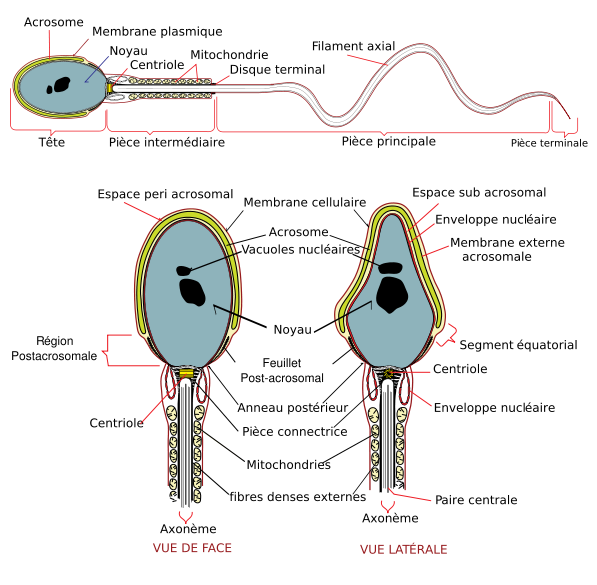
\includegraphics[scale=0.7]{figure/spermatozoide} 
  
  }
  
  \caption{Anatomie du spermatozoïde}\label{fig:spermatozoïde}
  \end{figure}
  
  \subsubsection{La tête}\label{la-tete}
  
  \subsubsection{Le flagelle}\label{le-flagelle}
  
  \subsection{Fonction du spermatozoïde}\label{fonction-du-spermatozoide}
  
  \section{L'infertilité masculine}\label{linfertilite-masculine}
  
  L'organisation mondiale de la santé définie l'infertilité comme étant :
  ``\emph{une pathologie du système reproductif définie par l'échec d'une
  grossesse clinique après 12 mois ou plus de rapports sexuels réguliers
  non protégés}''
  (\href{http://www.who.int/reproductivehealth/topics/infertility/definitions/en/}{\texttt{Who.int.\ 2013-03-19.\ Retrieved\ 2013-06-17}}).
  Environ 10-15\% des couples humains sont considérés infertiles. On
  estime que dans la moitié des cas, la cause sous-jacente est masculine.
  Les facteurs causaux sous-jacents de l'infertilité masculine peuvent
  être attribués à des toxines environnementales, des troubles systémiques
  tels que la maladie hypothalamo-hypophysaire, les cancers testiculaires
  et l'aplasie des cellules germinales. Les facteurs génétiques, y compris
  les aneuploïdies et les mutations de gènes uniques, contribuent
  également à l'infertilité masculine. Cependant, aucune cause n'est
  identifiée dans 10-20\% des cas.
  
  \subsection{Les différents phénotypes d'infertilité
  masculine}\label{les-differents-phenotypes-dinfertilite-masculine}
  
  \subsubsection{Liée à la quantité}\label{liee-a-la-quantite}
  
  \subsubsection{liée à la forme}\label{liee-a-la-forme}
  
  \subsubsection{liée à la mobilitée}\label{liee-a-la-mobilitee}
  
  \subsection{La génétique de
  l'infertilité}\label{la-genetique-de-linfertilite}
  
  \subsubsection{Les causes fréquentes}\label{les-causes-frequentes}
  
  \paragraph{Les microdélétions du chromosome
  Y}\label{les-microdeletions-du-chromosome-y}
  
  \paragraph{Anomalies chromosomiques}\label{anomalies-chromosomiques}
  
  \paragraph{Mutations CFTR}\label{mutations-cftr}
  
  \subsubsection{Les nouveaux gènes}\label{les-nouveaux-genes}
  
  \begin{center}\rule{0.5\linewidth}{\linethickness}\end{center}
  
  \section{Les techniques d'analyses
  génétiques}\label{les-techniques-danalyses-genetiques}
  
  \subsection{Les puces}\label{les-puces}
  
  \subsection{Le séquençage}\label{le-sequencage}
  
  \subsubsection{Le Sanger}\label{le-sanger}
  
  \subsubsection{Le NGS}\label{le-ngs}
  
  \begin{center}\rule{0.5\linewidth}{\linethickness}\end{center}
  
  \section{L'analyse bioinformatique}\label{lanalyse-bioinformatique}
  
  \subsection{L'analyse des données brut}\label{lanalyse-des-donnees-brut}
  
  \subsubsection{L'alignement}\label{lalignement}
  
  \subsubsection{L'appel des variants}\label{lappel-des-variants}
  
  \subsection{La priorisation des
  variants}\label{la-priorisation-des-variants}
  
  \chapter{Investigation génétique et physiologique de la
  globozoospermie}\label{globo}
  
  --\textgreater{}
  
  --\textgreater{}
  
  --\textgreater{}
  
  --\textgreater{}
  
  \chapter*{Conclusion}\label{conclusion}
  \addcontentsline{toc}{chapter}{Conclusion}
  
  \appendix
  
  \chapter{The First Appendix}\label{the-first-appendix}
  
  This first appendix includes all of the R chunks of code that were
  hidden throughout the document (using the \texttt{include\ =\ FALSE}
  chunk tag) to help with readibility and/or setup.
  
  \textbf{In the main Rmd file}
  
  \textbf{In Chapter \ref{ref-labels}:}
  
  \begin{Shaded}
  \begin{Highlighting}[]
  \CommentTok{# This chunk ensures that the thesisdown package is}
  \CommentTok{# installed and loaded. This thesisdown package includes}
  \CommentTok{# the template files for the thesis and also two functions}
  \CommentTok{# used for labeling and referencing}
  \NormalTok{if(!}\KeywordTok{require}\NormalTok{(devtools))}
    \KeywordTok{install.packages}\NormalTok{(}\StringTok{"devtools"}\NormalTok{, }\DataTypeTok{repos =} \StringTok{"http://cran.rstudio.com"}\NormalTok{)}
  \NormalTok{if(!}\KeywordTok{require}\NormalTok{(dplyr))}
      \KeywordTok{install.packages}\NormalTok{(}\StringTok{"dplyr"}\NormalTok{, }\DataTypeTok{repos =} \StringTok{"http://cran.rstudio.com"}\NormalTok{)}
  \NormalTok{if(!}\KeywordTok{require}\NormalTok{(ggplot2))}
      \KeywordTok{install.packages}\NormalTok{(}\StringTok{"ggplot2"}\NormalTok{, }\DataTypeTok{repos =} \StringTok{"http://cran.rstudio.com"}\NormalTok{)}
  \NormalTok{if(!}\KeywordTok{require}\NormalTok{(ggplot2))}
      \KeywordTok{install.packages}\NormalTok{(}\StringTok{"bookdown"}\NormalTok{, }\DataTypeTok{repos =} \StringTok{"http://cran.rstudio.com"}\NormalTok{)}
  \NormalTok{if(!}\KeywordTok{require}\NormalTok{(thesisdown))\{}
    \KeywordTok{library}\NormalTok{(devtools)}
    \NormalTok{devtools::}\KeywordTok{install_github}\NormalTok{(}\StringTok{"ismayc/thesisdown"}\NormalTok{)}
    \NormalTok{\}}
  \KeywordTok{library}\NormalTok{(thesisdown)}
  \NormalTok{flights <-}\StringTok{ }\KeywordTok{read.csv}\NormalTok{(}\StringTok{"data/flights.csv"}\NormalTok{)}
  \end{Highlighting}
  \end{Shaded}
  
  \chapter{The Second Appendix, for
  Fun}\label{the-second-appendix-for-fun}
  
  \backmatter
  
  \chapter*{References}\label{references}
  \addcontentsline{toc}{chapter}{References}
  
  \noindent
  
  \setlength{\parindent}{-0.20in} \setlength{\leftskip}{0.20in}
  \setlength{\parskip}{8pt}
  
  \hypertarget{refs}{}
  \hypertarget{ref-Clermont1963}{}
  Clermont, Y. (1963). The cycle of the seminiferous epithelium in man.
  \emph{American Journal of Anatomy}, \emph{112}(1), 35--51.
  \url{http://doi.org/10.1002/aja.1001120103}
  
  \hypertarget{ref-Clermont1966}{}
  Clermont, Y. (1966). Renewal of spermatogonia in man. \emph{American
  Journal of Anatomy}, \emph{118}(2), 509--524.
  \url{http://doi.org/10.1002/aja.1001180211}
  
  \hypertarget{ref-Escalier1991}{}
  Escalier, D., Gallo, J.-M., Albert, M., Meduri, G., Bermudez, D., David,
  G., \& Schrevel, J. (1991). Human acrosome biogenesis: immunodetection
  of proacrosin in primary spermatocytes and of its partitioning pattern
  during meiosis. \emph{Development}, \emph{113}, 779--788. Retrieved from
  \url{http://dev.biologists.org/content/develop/113/3/779.full.pdf}
  
  \hypertarget{ref-Gnessi1997}{}
  Gnessi, L., Fabbri, A., \& Spera, G. (1997). Gonadal Peptides as
  Mediators of Development and Functional Control of the Testis: An
  Integrated System with Hormones and Local Environment
  \textless{}sup\textgreater{}1\textless{}/sup\textgreater{}.
  \emph{Endocrine Reviews}, \emph{18}(4), 541--609.
  \url{http://doi.org/10.1210/edrv.18.4.0310}
  
  \hypertarget{ref-Goossens2013}{}
  Goossens, E., \& Tournaye, H. (2013). Adult Stem Cells in the Human
  Testis. \emph{Seminars in Reproductive Medicine}, \emph{31}(01),
  039--048. \url{http://doi.org/10.1055/s-0032-1331796}
  
  \hypertarget{ref-Hamilton1987}{}
  Hamilton, D., Waites, G. M. H., Special Programme of Research, D.,
  Family Health International (Organization), \& World Health
  Organization. (1987). \emph{Cellular and molecular events in
  spermiogenesis} (p. 334). Cambridge University Press.
  
  \hypertarget{ref-Johnson1980}{}
  Johnson, L., Petty, C. S., \& Neaves, W. B. (1980). A comparative study
  of daily sperm production and testicular composition in humans and rats.
  \emph{Biology of Reproduction}, \emph{22}(5), 1233--43. Retrieved from
  \url{http://www.ncbi.nlm.nih.gov/pubmed/7417656}
  
  \hypertarget{ref-KIERSZENBAUM1994}{}
  Kierszenbaum, A. L. (1994). Mammalian Spermatogenesis in Vivo and in
  Vitro : A Partnership of Spermatogenic and Somatic Cell Lineages*.
  \emph{Endocrine Reviews}, \emph{15}(1), 116--134.
  \url{http://doi.org/10.1210/edrv-15-1-116}


  % Index?

\end{document}

